\chapter{Experimento \& Análise}
\label{cap6}



Apartir dos dados coletados, foi realizado uma análise dos dados seguindo os critérios levantados durante a proposta do atual trabalho.
%
Tal análise visa compreender o consumo de recurso usado pelas arquiteturas com base em suas características específicas.



Cada caso de análise é dividido em experimentos, na qual cada experimento tem o objetivo de analisar um conjunto de recursos dado alguma situação.
%
Nesse sentido, faz sentido agrupar tais experimentos, agrupados na Sessão~\ref{sec:experimentos}, para posterior comparação.



%ccm todo gráfico precisa responder a alguma pergunta.
% 1- Formular a pergunta com base no que definiu no Cap.4
% 2- quem está envolvido, quais são os parâmetros, quais são constantes
% 3- Descrever o perfil/modus operandi do experimento
% 4- Mostra a figura
% 5- Analisa os resultados com base na expectativa no Cap.4 (foi similar, diferente, por quê?)
% 6 - Precisa manter em mente que as figuras devem manter uma escala para poder comparar entre diferentes arquiteturas


\section{Experimentos}
\label{sec:experimentos}



Cada experimento utiliza as arquiteturas Rudy, Salz e Willson.
%
Cada arquitetura é executada no mesmo ambiente, isolados por momentos diferentes.
%
Para cada arquitetura, é realizado três execuções com os mesmos parâmetros.
%
Em cada execução, o seguinte protocolo é seguido:



\begin{enumerate}
 \item Inicio dos serviços do banco de dados.
 \item Inicio dos serviços de jogo.
 \item Inicio dos clientes.
 \item Clientes são escalados de 1 em 1 até 100, com 30 segundos de intervalo.
 \item Todos os serviços em todos os ambientes são removidos, mantendo somente os dados capturados.
\end{enumerate}



A partir de tais execuções, os dados são capturados, processados e analisados.
%
Durante as execuções, os dados de latência foram estáveis entre 5ms e 15ms, dessa forma foram ignorados como um experimento a parte.



\subsection{Consumo de \ac{cpu}}



Este experimento visa analisar o consumo de \ac{cpu} unitariamente, em relação ao número de jogadores simultâneos.
%
Espera-se que o seu crescimento seja linear seguindo o crescimento de jogadores concorrentes.
%
Neste contexto existem os seguintes valores:



\begin{itemize}
    \item Jogadores simultâneos: Variável capturada a partir do microsserviço de jogo.
    \item Consumo de \ac{cpu}: Variável capturada a partir do monitor de recursos do Docker.
\end{itemize}

Dado este contexto, os dados de consumo de \ac{cpu} obtidos são visíveis na Figura~\ref{fig:experimento_cpu}.



\begin{figure}[htb!]
    \caption{Consumo de \ac{cpu} das arquiteturas}
    \label{fig:experimento_cpu}

    \begin{subfigure}{.5\textwidth}
        \centering
        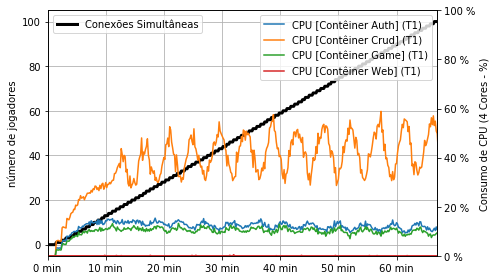
\includegraphics[width=.95\linewidth]{figuras/testes/r_cpu_game.png}
        \caption{Microsserviços da arquitetura Rudy}
        \label{fig:r_cpu_game}
    \end{subfigure}%
    \begin{subfigure}{.5\textwidth}
        \centering
        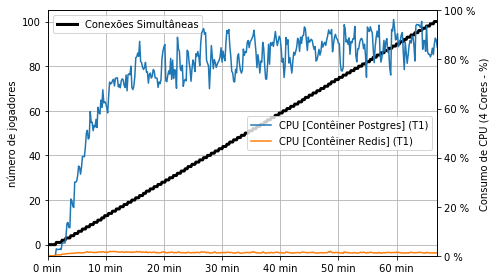
\includegraphics[width=.95\linewidth]{figuras/testes/r_cpu_db.png}
        \caption{Banco de Dados da arquitetura Rudy}
        \label{fig:r_cpu_db}
    \end{subfigure}%

    \begin{subfigure}{.5\textwidth}
        \centering
        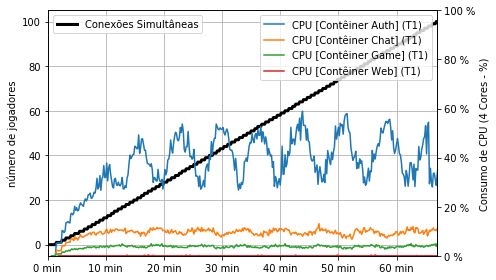
\includegraphics[width=.95\linewidth]{figuras/testes/s_cpu_game.png}
        \caption{Microsserviços da arquitetura Salz}
        \label{fig:s_cpu_game}
    \end{subfigure}%
    \begin{subfigure}{.5\textwidth}
        \centering
        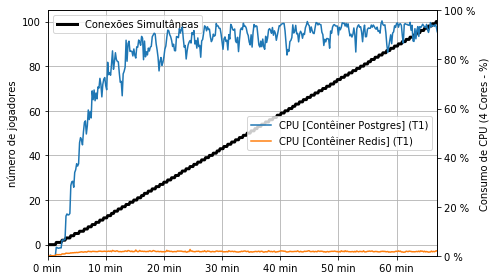
\includegraphics[width=.95\linewidth]{figuras/testes/s_cpu_db.png}
        \caption{Banco de Dados da arquitetura Salz}
        \label{fig:s_cpu_db}
    \end{subfigure}%

        \begin{subfigure}{.5\textwidth}
        \centering
        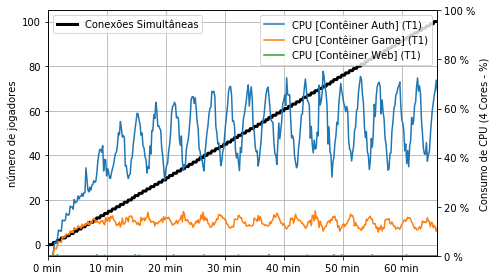
\includegraphics[width=.95\linewidth]{figuras/testes/w_cpu_game.png}
        \caption{Microsserviços da arquitetura Willson}
        \label{fig:w_cpu_game}
    \end{subfigure}%
    \begin{subfigure}{.5\textwidth}
        \centering
        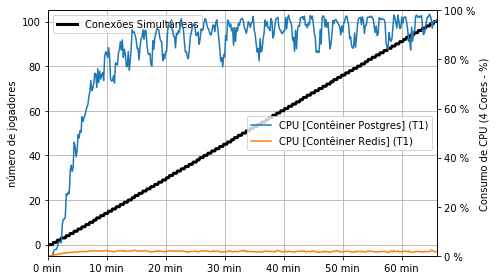
\includegraphics[width=.95\linewidth]{figuras/testes/w_cpu_db.png}
        \caption{Banco de Dados da arquitetura Willson}
        \label{fig:w_cpu_db}
    \end{subfigure}%

    Fonte: O próprio autor.
\end{figure}



A Figura~\ref{fig:experimento_cpu} exibe todos os resultados obtidos sobre consumo de \ac{cpu} das arquiteturas de microsserviços, em sua primeira execução.
%
A segunda e terceira execução obtiveram resultados equivalentes.



Uma característica notória sobre os bancos de dados utilizados é a disparidade entre o consumo de \ac{cpu} do banco de dados permanente e temporário, exibida nas Figuras~\ref{fig:r_cpu_db}, \ref{fig:s_cpu_db} e \ref{fig:w_cpu_db}.
%
Esta característica é relacionada a natureza do armazenamento dos dados, sendo o PostgreSQL com características \ac{acid} e o Redis sendo um banco de dados chave-valor em memória.
%
Pela diferença de natureza entre os bancos, espera-se um aumento do consumo de \ac{cpu} por parte do banco de dados PostgreSQL.

Em relação ao consumo de recursos por parte dos microsserviços, pode-se selecionar os maiores e menores consumidores de recurso dos testes.
%
Esta listagem está disponível na Tabela~\ref{tab:cpu_consumo_max_min}.



\begin{table}[htb!]
\centering
\begin{adjustbox}{max width=\textwidth}
\caption{Maiores e menores consumidores de \ac{cpu}.}
\label{tab:cpu_consumo_max_min}
\begin{tabular}{|l|l|l|}

\hline

Arquitetura & Maior Consumidor & Menor Consumidor \\ \hline

Rudy        & rcrud            & rweb             \\ \hline

Salz        & sauth            & sweb             \\ \hline

Willson     & wauth             & wweb             \\ \hline

\end{tabular}
\end{adjustbox}

Fonte: O próprio autor.
\end{table}



Conforme exibido na Tabela~\ref{tab:cpu_consumo_max_min}, os maiores consumidores de \ac{cpu} são os serviços que realizam papel de conexão com banco de dados e/ou autenticação.
%
Antagonicamente, os serviços Web são os menores consumidores de \ac{cpu}.



Para o caso dos maiores consumidores de \ac{cpu}, exibidos na Tabela~\ref{tab:cpu_consumo_max_min}, os serviços \textit{sauth} e \textit{wauth} são usados para realizar conexão ao PostgreSQL / Redis ou realizando operações da biblioteca \textit{bcrypt} (autenticação).
%
Entretanto, o serviço \textit{rcrud} é responsável por monopolizar o acesso ao banco, não realizando operações da biblioteca \textit{bcrypt}.
%
Dessa forma, o maior fator de consumo de recursos em tais serviços é a conexão com o banco de dados.



Para o caso dos menores consumidores de \ac{cpu}, nota-se que é ocupado pelo microsserviço Web.
%
Tal microsserviço é pouco utilizado, sendo chamado somente para a criação da conta e personagem.
%
Dessa forma, ele não respeita o crescimento linear de jogadores simultâneos.



Ainda existe uma diferença de consumo de \ac{cpu} entre os serviços \textit{sauth} \textit{wauth}, listados na Tabela~\ref{tab:cpu_consumo_max_min} na coluna de maiores consumidores.
%
Nota-se uma diferença de 20\% no consumo de recursos, exibidos nas Figuras~\ref{fig:s_cpu_game} e~\ref{fig:w_cpu_game}.
%
Este aumento de consumo de recursos da arquitetura Willson é relação direta da liberação de recursos na estratégia de manter o sistema de \textit{chat} junto ao microsserviço de jogo.
%
Esta mesma característica pode ser comparada ao microsserviço \textit{rcrud} visível na Figura~\ref{fig:r_cpu_game}, visto que em ambos microsserviços citados, o motivo de sua elevada carga \ac{cpu} é o acesso ao banco de dados.



\subsection{Consumo de Memória}


Este experimento visa analisar o consumo de memória unitariamente, em relação ao número de jogadores simultâneos.
%
Espera-se que o seu crescimento seja linear seguindo o crescimento de jogadores concorrentes.
%
Neste contexto existem os seguintes valores:



\begin{itemize}
    \item Jogadores simultâneos: Variável capturada a partir do microsserviço de jogo.
    \item Consumo de memória: Variável capturada a partir do monitor de recursos do Docker.
\end{itemize}

Dado este contexto, os dados de consumo de memória obtidos são visíveis na Figura~\ref{fig:experimento_mem}.



\begin{figure}[htb!]
    \caption{Consumo de memória das arquiteturas}
    \label{fig:experimento_mem}

    \begin{subfigure}{.5\textwidth}
        \centering
        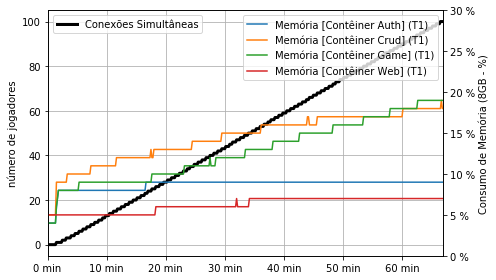
\includegraphics[width=.95\linewidth]{figuras/testes/r_mem_game.png}
        \caption{Microsserviços da arquitetura Rudy}
        \label{fig:r_mem_game}
    \end{subfigure}%
    \begin{subfigure}{.5\textwidth}
        \centering
        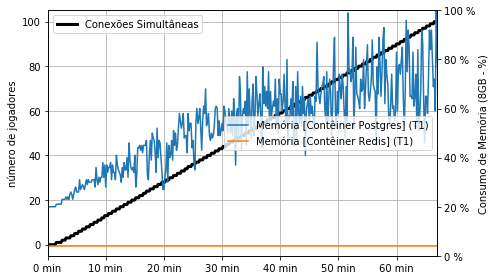
\includegraphics[width=.95\linewidth]{figuras/testes/r_mem_db.png}
        \caption{Banco de Dados da arquitetura Rudy}
        \label{fig:r_mem_db}
    \end{subfigure}%

    \begin{subfigure}{.5\textwidth}
        \centering
        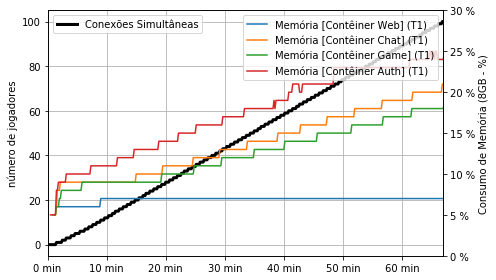
\includegraphics[width=.95\linewidth]{figuras/testes/s_mem_game.png}
        \caption{Microsserviços da arquitetura Salz}
        \label{fig:s_mem_game}
    \end{subfigure}%
    \begin{subfigure}{.5\textwidth}
        \centering
        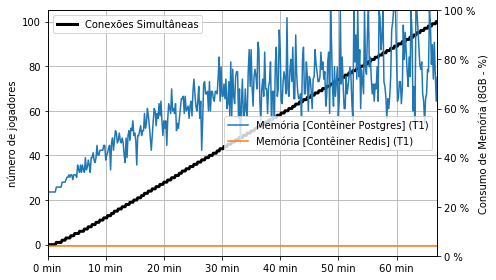
\includegraphics[width=.95\linewidth]{figuras/testes/s_mem_db.png}
        \caption{Banco de Dados da arquitetura Salz}
        \label{fig:s_mem_db}
    \end{subfigure}%

        \begin{subfigure}{.5\textwidth}
        \centering
        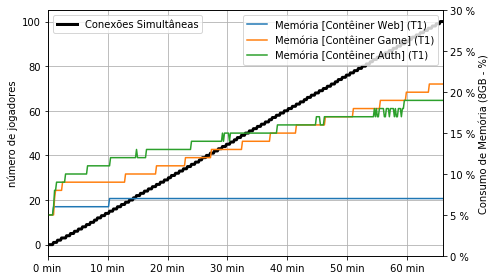
\includegraphics[width=.95\linewidth]{figuras/testes/w_mem_game.png}
        \caption{Microsserviços da arquitetura Willson}
        \label{fig:w_mem_game}
    \end{subfigure}%
    \begin{subfigure}{.5\textwidth}
        \centering
        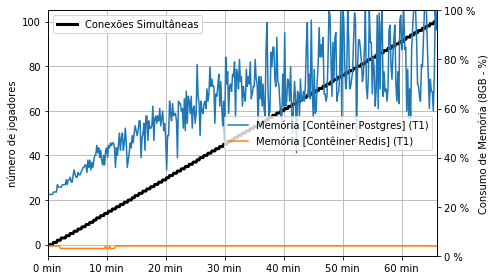
\includegraphics[width=.95\linewidth]{figuras/testes/w_mem_db.png}
        \caption{Banco de Dados da arquitetura Willson}
        \label{fig:w_mem_db}
    \end{subfigure}%

    Fonte: O próprio autor.
\end{figure}

\subsection{Rede - Entrada / Saída}

\begin{figure}[htb!]
    \caption{Consumo de rede das arquiteturas}
    \label{fig:experimento_net}

    \begin{subfigure}{.5\textwidth}
        \centering
        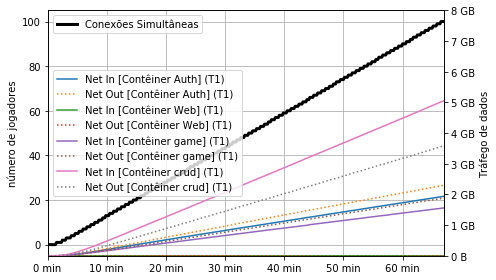
\includegraphics[width=.95\linewidth]{figuras/testes/r_net_game.png}
        \caption{Microsserviços da arquitetura Rudy}
        \label{fig:r_net_game}
    \end{subfigure}%
    \begin{subfigure}{.5\textwidth}
        \centering
        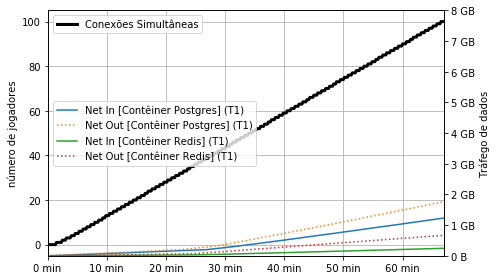
\includegraphics[width=.95\linewidth]{figuras/testes/r_net_db.png}
        \caption{Banco de Dados da arquitetura Rudy}
        \label{fig:r_net_db}
    \end{subfigure}%

    \begin{subfigure}{.5\textwidth}
        \centering
        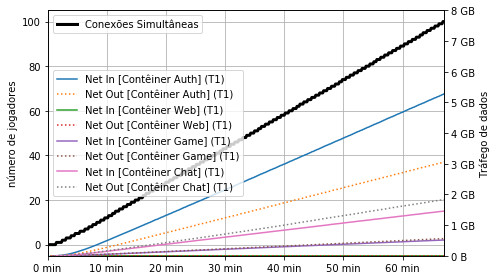
\includegraphics[width=.95\linewidth]{figuras/testes/s_net_game.png}
        \caption{Microsserviços da arquitetura Salz}
        \label{fig:s_net_game}
    \end{subfigure}%
    \begin{subfigure}{.5\textwidth}
        \centering
        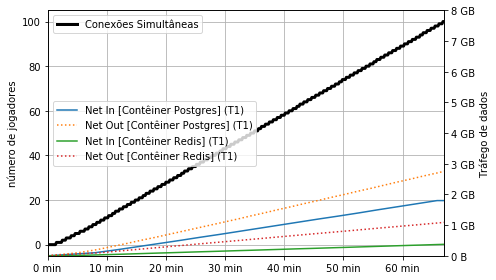
\includegraphics[width=.95\linewidth]{figuras/testes/s_net_db.png}
        \caption{Banco de Dados da arquitetura Salz}
        \label{fig:s_net_db}
    \end{subfigure}%

        \begin{subfigure}{.5\textwidth}
        \centering
        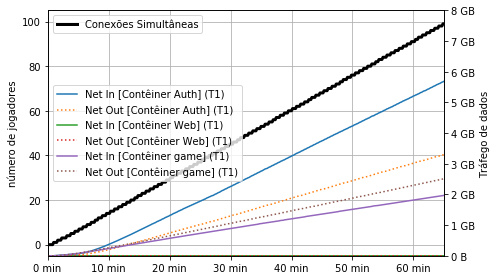
\includegraphics[width=.95\linewidth]{figuras/testes/w_net_game.png}
        \caption{Microsserviços da arquitetura Willson}
        \label{fig:w_net_game}
    \end{subfigure}%
    \begin{subfigure}{.5\textwidth}
        \centering
        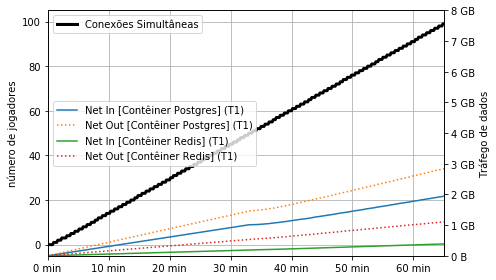
\includegraphics[width=.95\linewidth]{figuras/testes/w_net_db.png}
        \caption{Banco de Dados da arquitetura Willson}
        \label{fig:w_net_db}
    \end{subfigure}%

    Fonte: O próprio autor.
\end{figure}

\subsection{Tempo de resposta das Requisições}

\section{Análise}
